% biography section
% 
% If you have an EPS/PDF photo (graphicx package needed) extra braces are
% needed around the contents of the optional argument to biography to prevent
% the LaTeX parser from getting confused when it sees the complicated
% \includegraphics command within an optional argument. (You could create
% your own custom macro containing the \includegraphics command to make things
% simpler here.)
\begin{IEEEbiography}[{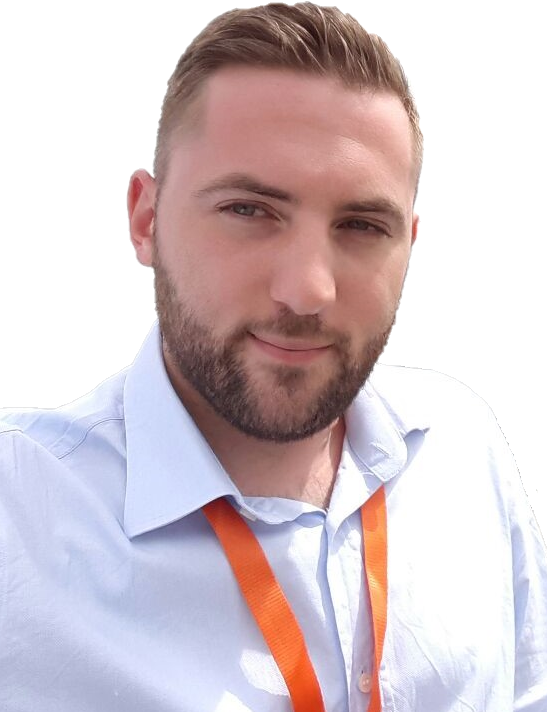
\includegraphics[width=1in,height=1.25in,clip,keepaspectratio]{bioImg/DomenicoChiaradia.png}}]{Domenico Chiaradia}
received the B.S. and M.S. degrees with honours in control theory and automation engineering from the Polytechnic University of Bari, Italy, in 2011 and 2014 respectively.  He is currently pursuing the Ph.D. degree in robotics engineering at Perceptual Robotics (PERCRO) Laboratory, TeCIP Institute, Sant'Anna School of Advanced Studies, Pisa, Italy.
His research interest includes control of rigid and soft exoskeletons for assistance and rehabilitation, torque control, control of haptic interfaces and physical human-robot interaction.
%
\end{IEEEbiography}

% if you will not have a photo at all:
\begin{IEEEbiography}[{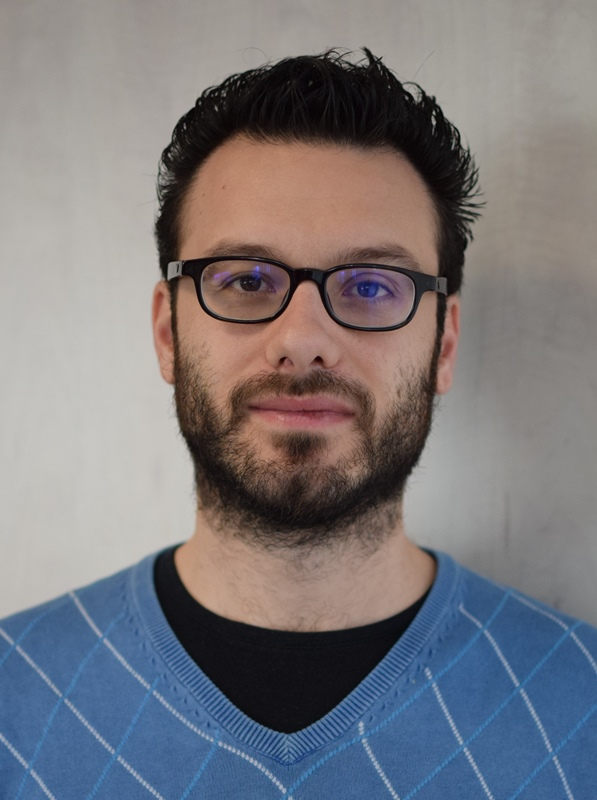
\includegraphics[width=1in,height=1.25in,clip,keepaspectratio]{bioImg/MassiSmall2.jpg}}]{Massimiliano Solazzi} (Eng., Ph.D.) is Assistant Professor in Applied Mechanics at the Sant'Anna School of Advanced Studies in Pisa, Italy. He carries out his research at the Percro laboratory - TeCIP.  In 2010 he received the PhD Degree in Innovative Technologies from the Sant'Anna School of Advanced Studies. 
His research interests concerns: the design of robotic interfaces for virtual reality, teleoperation and rehabilitations, and the psychophysical validation of HMI.
\end{IEEEbiography}


\begin{IEEEbiography}[{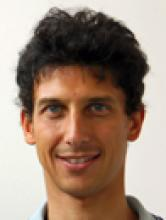
\includegraphics[width=1in,height=1.25in,clip,keepaspectratio]{bioImg/r_vertechy.jpg}}]{Rocco Vertechy} (Eng., Ph.D.)  is Associate Professor at the Industrial Engineering Department of the School of Engineering and Architecture of the University of Bologna in Italy, where he leads the group on advanced actuation technologies and renewable energy robotic systems. He is Mechanical Engineer (2001) and PhD in Mechanics of Machines (2005). He was: Research Assistant at the Department of Mechanical Engineering, University of Canterbury (New Zealand); Visiting Researcher at the Robotics Locomotion Laboratory, Stanford University (California); Contract Professor at the University of Bologna; Assistant Professor at the Perceptual Robotics Laboratory of the Scuola Superiore Sant’Anna (Italy).
	
\end{IEEEbiography}

% insert where needed to balance the two columns on the last page with
% biographies
%\newpage

\begin{IEEEbiography}[{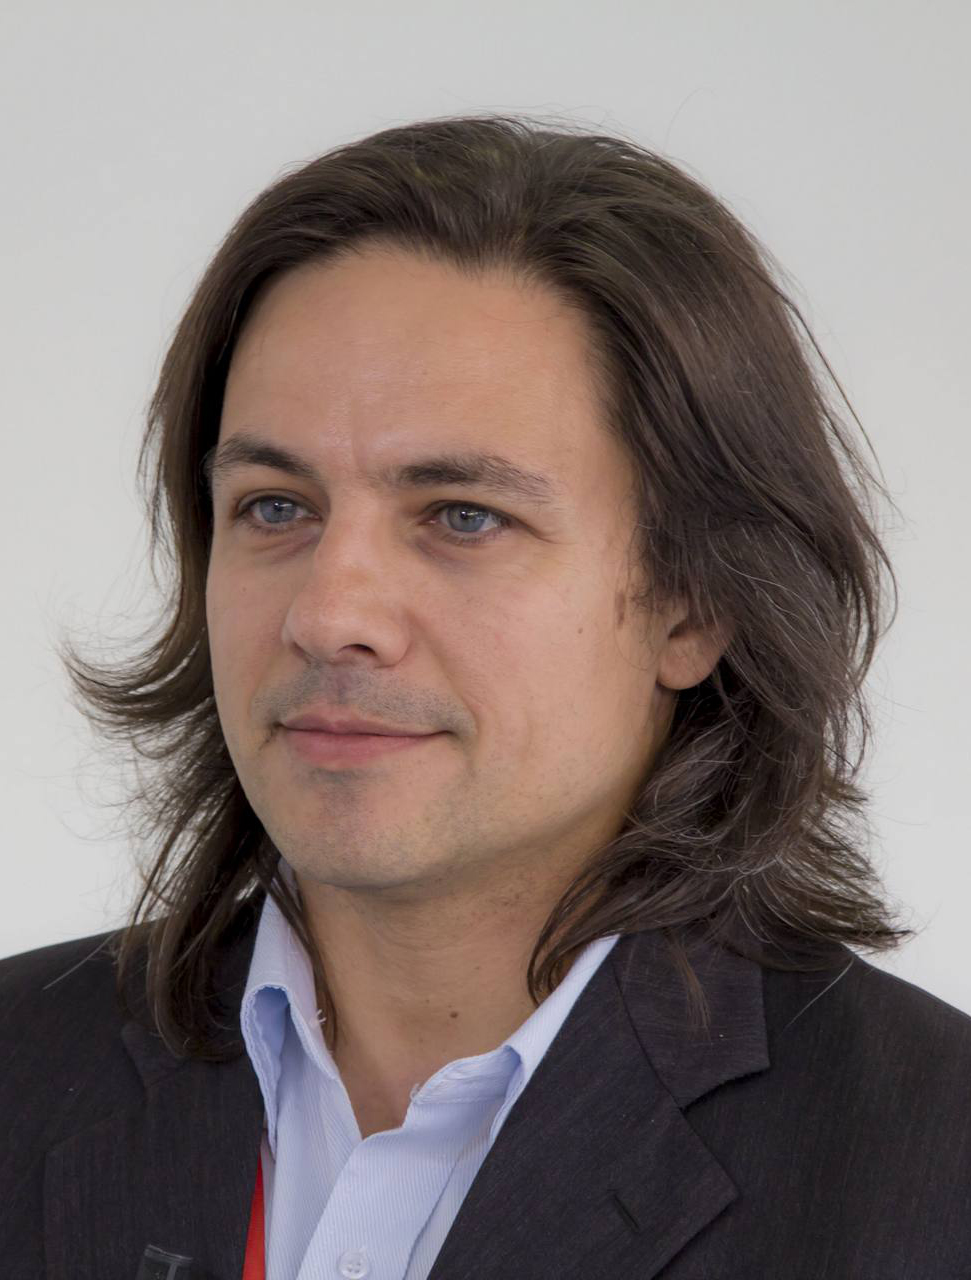
\includegraphics[width=1in,height=1.25in,clip,keepaspectratio]{bioImg/frisoli3.jpg}}]{Antonio Frisoli} (Eng., PhD) is Professor of Robotics and Mechanical Engineering at the Sant'Anna School of Advanced Studies, Pisa-Italy, where he is head of the Human-Robot Interaction area at PERCRO laboratory of TeCIP Institute. He received his PhD (2002) with honors in Industrial and Information Engineering from the Sant'Anna School of Advanced Studies, Italy and the MSc (1998) in Mechanical Engineering, minor Robotics, from University of Pisa-Italy.  He has been chair of the IEEE Technical Committee on Haptics, the general chair of the Eurohaptics 2018 conference in Pisa and Human-Machine Interaction summer school HMISS 2017. In the field of robotics and haptics he acts as associated editor in numerous international conferences, such as IEEE Worldhaptics, IEEE Roman, IEEE Haptic Symposium among many others, and journals, such as IEEE Robotics and Automation Letters and MIT Press Presence.

%Antonio Frisoli’s research interests are in the field on design and control of haptic devices and robotic systems, rehabilitation robotics and human motor control, virtual reality, advanced human computer interfaces for  training, Brain Computer Interfaces. Currently he is studying new designs for  exoskeletons systems, portable fingertip haptics and new brain-robot interfaces.
%He is author of more than 200 papers in peer-reviewed international conferences and scientific journals.

\end{IEEEbiography}